\documentclass[a4paper, 11pt]{article}

\usepackage[czech]{babel}
\usepackage[utf8]{inputenc}
\usepackage[left=2cm, top=3cm, text={17cm, 24cm}]{geometry}
\usepackage{times}
\usepackage[unicode]{hyperref}
\usepackage{indentfirst}
\usepackage{graphics}
\usepackage{fancyvrb}
\usepackage{listings}
\usepackage{xcolor}
\lstset{basicstyle=\footnotesize\ttfamily,breaklines=true}
\lstset{framextopmargin=50pt,frame=none}
\hypersetup{colorlinks = true, hypertexnames = false}

\renewcommand*\contentsname{Obsah}

\begin{document}

	\begin{titlepage}
		\begin{center}
			\LARGE\textsc{Vysoké učení technické v~Brně} \\
			\Large\textsc{Fakulta informačních technologií}\\
			\vspace{\stretch{0.382}}
			\large{IFJ - Projektová dokumentace} \\
			\LARGE{Implementace překladače jazyka IFJ22} \\
			\vspace{0.2cm}
			\large{Tým "Tým xkalis03", varianta BVS}
			\vspace{\stretch{0.618}}
		\end{center}

		\Large{\hspace*{-0.6cm}Autoři: \hfill (v) \hspace{0.1cm} Vojtěch Kališ (xkalis03)} \hspace{0.97cm} 25\% \\
		\Large{\hspace*{\fill} Jan Lutonský (xluton02)} \hspace{0.82cm} 25\% \\
		\Large{\hspace*{\fill} Jan Salaš (xsalas02)} \hspace{1.73cm} 25\% \\
		\Large{\hspace*{\fill} Lucie Hlaváčová (xhlava60)} \hspace{0.1cm} 25\% \\ \\
		\Large{Implementovaná rozšíření:  \hspace*{1cm} FUNEXP} \hfill
	\end{titlepage}

%%% TOC
	\tableofcontents

%%%
	\newpage
	\section{Úvod}
	Cílem tohoto projektu bylo vytvořit překladač implementovaný v~jazyce C, který ze standartního vstupu načte vstupní kód napsaný v~jazyce IFJ22, přeloží
	jej do cílového jazyka IFJcode22 a výskedek pak vypíše na standartní výstup. Jazyk IFJ22 vznikl jako obdoba jazyka PHP. 
%%%
	\section{Implementace}
	Celý překladač jsme si rozdělili na více dílčích problémů, jejichž funkčnost byla individuálně testována. Tyhle dílčí problémy byly nadále vzájemně 
	propojovány a opět testována jejich funkčnost.
	\subsection{Lexikální analyzátor}
	\subsection{Syntaktický analyzátor}
    Syntaktický analyzátor je závislý na lexykalním a vála jeho funkce aby získal nový token. Tokeny
    jsou předávány přes strukturu context která slouží pro sdílení dat mezi částmi překladače.
    Rozhodli jsme se implementovat syntaktickou analýzu metodou rekurzivního sestupu. Při návrhu gramatiky
    jsme narazili na problém kdy pravidlo pro příkaz přiřazení výrazu do proměné kolidovalo s
    výrazem bez přizazení který osahuje pouze identifikátor z toho to důvodu jsme se rozhodli 
    přemístit syntaktickoou analízu příkazu přiřazení do precedenční syntaktické analýzy. 
    Na další problém jsme narazili při volání funkcí, protože jsme se rozhodli implementovat 
    rozšíření FUNEXP tak jsme museli zajistit, že funkce je možné analyzovat i uprostřed výrazů 
    a jelikož nám přišlo složité přepínat mezi syntaktickou analýzou rekurzivním sestupem a syntaktickou 
    analyzou precednční tabulkou tak jsme se rozhodli přemístit volání funkce jen do syntaktické analýzi precedenřní
    tabulkou. Analyzátor paři svém fungovaní tvoří abstraktní \ignore{TODO link} syntaktický strom který je dále spracováván 
    dalšími části překladače.

	\subsubsection{Precedenční syntaktický analyzátor}
    Slouží ke zpracování výrazů, přikazu přiřazení do proměné a volání funkce. Při tvorbě precedenční tabulky jsem si 
    všiml, že operátori je možné sjednotit do množin se stejnou precedencí díky tomu jsem mohl tabulku zmenšit. Precedenční
    analyzátor analyzuje vstupní tokeny, ziskané z lexikálního analyzátoru přes strukturu context, dokud nenarazý na první
    token který se nesmí vyskytovat ve výrazu, volání funkce nebo v příkazu přiřazení. Tento token není zkonzumován a je 
    ponechán v struktůře context pro další zpracování Syntaktickým analizátorem metodou rekurzivní sestup. Redukce gramatických
    pravidel na zásobníku Precedenční syntaktycké analýzi probíhají pomocí stavového automatu posaným tímto diagramem. \ignore{TODO link}
    \ignore{TODO vložit gram pravidla pro redukce}


	\subsection{Sémantický analyzátor}
	\label{semantic}
	Sémantický analyzátor provádí sémantickou analýzu nad vstupním programem, a je obsažen v souboru \textit{semantic\.c}; jeho hlavičkový soubor pak 
	analogicky nese název \textit{semantic\.h}. Sémantický analyzátor pracuje převážně s Globální tabulkou symbolů (využívající implementace 
	\hyperref[symtab]{Tabulky symbolů} a Abstraktním syntaktickým stromem (dále jen ASS). Očekává se korektní naplnění ASS v rámci syntaktické analýzy. Na 
	začátku své funkce sémantický analyzátor inicializuje Globální tabulku symbolů, projde ASS a vyhledá v něm všechny definice funkcí, jež vloží jakožto nody s 
	typem \textit{function} do Globální tabulky symbolů; možné parametry definované při deklaraci funkce zase vloží do Lokální tabulky symbolů dané funkce 
	jakožto nody s typem \textit{variable}. Do Globální tabulky symbolů jsou také vloženy deklarace vestavěných funkcí (zavoláním funkce ), společně s funkcí 
	nazvanou ":b" sloužící jako hlavní tělo programu (\textit{body}).

	Jakmile je vše připraveno, Sémantický analyzátor vstoupí do funkce \textit{AST\_DF\_traversal}, plnící funkci hlavní smyčky, která prochází již zmíněný AST 
	do hloubky a v rámci switch case-u pak hledá AST nody, jejichž sémantickou korektnost je třeba prověřit; jakmile nějakou takovou nodu najde, spustí nad ní 
	speciální funkci zabývající se prověřením sémantické korektnosti toho konkrétního typu AST nody. V případě, že je nalezena sémantická chyba, program 
	ukončí svou činnost, vypropaguje kód odpovídající nalezené chybě, a zaručí, že dojde ke kompletnímu uvolnění veškeré alokované paměti.
	\subsection{Generátor cílového kódu}
%%%
	\section{Speciální datové struktury}
    \subsection{Abstraktní syntaktický strom}
    Je implementován N-arním stromem\ignore{TODO link na wiki(M-ary tree)} tento strom je tvořen při syntaktické analýze a slouží jako vnitřní reprazentace
    vstupního kódu. Tento strom je ze syntektické analýzi předávan do sémantické analýzi kde je dále zpracováván po sémantické analýze je strom předán
    generátoru kódu který strom projde a generuje úseky kódu v závislosti na uzlech stromu. N-arní strom nám zjednodušil spracování zřetězených gramatických
    pravidel jako například seznam parametrů při definici funkce nebo seznam parametrů při volání funkce. \ignore{TODO obrazki AST pro každé pravidlo}

    \subsection{Generický zásobník}
    Je implementován pomocí dynamického pole ukazatelů na void. Při přidávání prvků na zásobník může dojít místo v dynamickém poli v takovém případě je k poli přialokováno 
    24 volných slotů zásobníku pomocí funkce realloc. Zvolil jsem přialokovávat 24 položek, protože mi to přišlo dostatečné ale nemohu to podložit žádným měřením
    nebo testy.
    
    \subsection{Zásobník pro precedenční syntaktickou analyzu}
    Je přetypvaná struktůra generického zásobníku. Pro tento zásobník byli vytvořeny funkce které správně přetipují vstupy a výstupy tak aby bylo možné volat funkce
    generického zásobníku. Samotný zásobník slouží pro ukládání uzlů syntaktického stromu které jsou následně redukovány precedenčním syntaktickým analyzátorem.

	\subsection{Tabulka symbolů}
	\label{symtab}
	Tabulka symbolů byla implementována jako binární vyhledávací strom, což bylo i nárokem naší varianty zadání. Téměř celá tabulka symbolů je napsána 
	nerekurzivním (tedy iterativním) postupem, a to především z důvodu snížení časové komplexity na úkor složitější implementace. Tabulka symbolů je 
	využívána \hyperref[semantic]{Sémantickým analyzátorem} pro vytvoření Globální tabulky symbolů a její využití je již popsáno v rámci jeho popisu.
	\subsection{Obousměrně vázaný seznam}
	Implementaci obousměrně vázaného seznamu lze najít v souboru \textit{dll.c}, a odpovídající hlavičkový soubor pak pod názvem \textit{dll.h}. Obousměrně 
	vázaný seznam je v projektu využíván ve struktuře nody Tabulky symbolů, a to pro účely snadného uchování názvů argumentů vkládaných funkcí.
	\subsection{ADT \#3}
	\subsection{...}
%%%
	\section{Práce v týmu}
	Na projektu jsme začali pracovat ihned po zveřejnění zadání, a to jeho prostudováním a domluvením první schůzky, v rámci které byla vypracována prvotní 
	verze pravidel LL-gramatiky, a LL tabulka. Obojí se ještě v čase dalších několika týdnů upravovalo v případě nalezení chyby, až se nakonec vše ustálilo do 
	konečné podoby, prezentované v tomhle dokumentě a dohledatelné na jeho \hyperref[gram]{konci}.
	
	Dále jsme si jednotlivé části rozdělili mezi sebe a pracovali na nich jako jednotlivci popřípadě dvojice. Stále probíhaly schůzky, například pro řešení 
	implementačních záležitostí a to především způsobu komunikace jednotlivých částí překladače, ovšem zvětšiny docházelo spíše k průběžnému testování 
	překladače jako celku a kontrole pokroku ve vývoji.
	\subsection{Komunikace}
	Pro komunikaci byla využita aplikace \textit{Discord}, kde byl vytvořen vlastní server na kterém pak probíhala veškerá vzájemná komunikace, ať už se 
	jednalo o komunikaci textovou, hovorové schůzky celotýmové i třeba v menším počtu, nebo sdílení materiálů, diagramů apod. 
	\subsection{Vzdálený repozitář}
	Jako vzdálený repozitář jsme zvolili Github, jenž nám umožnil sdílet mezi sebou zdrojové kódy dílčích úkolů a~navzájem si testovat nejen funkčnost 
	jednotlivých částí, ale i~překladač jako celek.
	\subsection{Rozdělení práce v týmu}
	Rozdělení: \hspace*{0.5cm} 	Jan Lutonský (xluton02): \hspace{0.1cm} Syntaktická analýza, Precedenční syntaktická analýza, Generátor \\
			\hspace*{5cm} cílového kódu, Speciální datové struktury, Testování\\
			\hspace*{2.25cm}	Vojtěch Kališ (xkalis03): \hspace{0.1cm} Sémantická analýza, Tabulka symbolů, Speciální datové struktury, \\
			\hspace*{5cm} Testování\\
			\hspace*{2.25cm}	Jan Salaš (xsalas02): \hspace{0.1cm} Lexikální analýza, Testování\\
			\hspace*{2.25cm}	Lucie Hlaváčová (xhlava60): \hspace{0.1cm} Lexikální analýza, Testování\\
%%%
	\section{Závěr}
	
%%%
	\newpage
	
	\begingroup\centering
	\section*{DKA pro konečný automat}
	\endgroup
	\vspace{1.8cm}
	\begin{figure}[h]
		\centering
		\hspace*{-1.2cm}
		\scalebox{0.5}{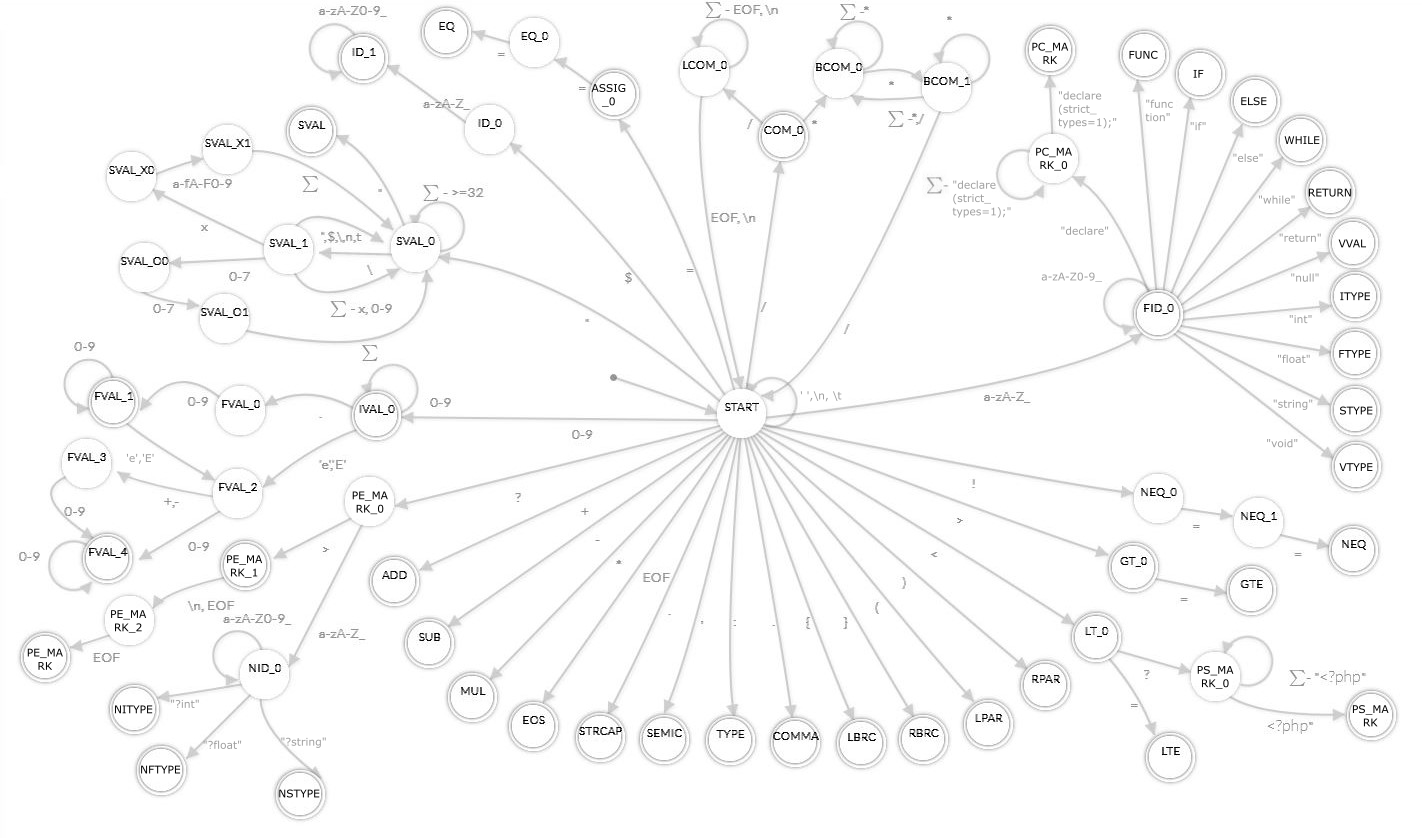
\includegraphics{diagrams/DKA.png}}
		\label{DKA}
	\end{figure}
%%%
	\newpage

	\begingroup\centering
	\section*{Precedenční tabulka}
	\endgroup
	\vspace{1.8cm}
	\begin{figure}[h]
		\centering
		\hspace*{-2cm}
		\scalebox{0.7}{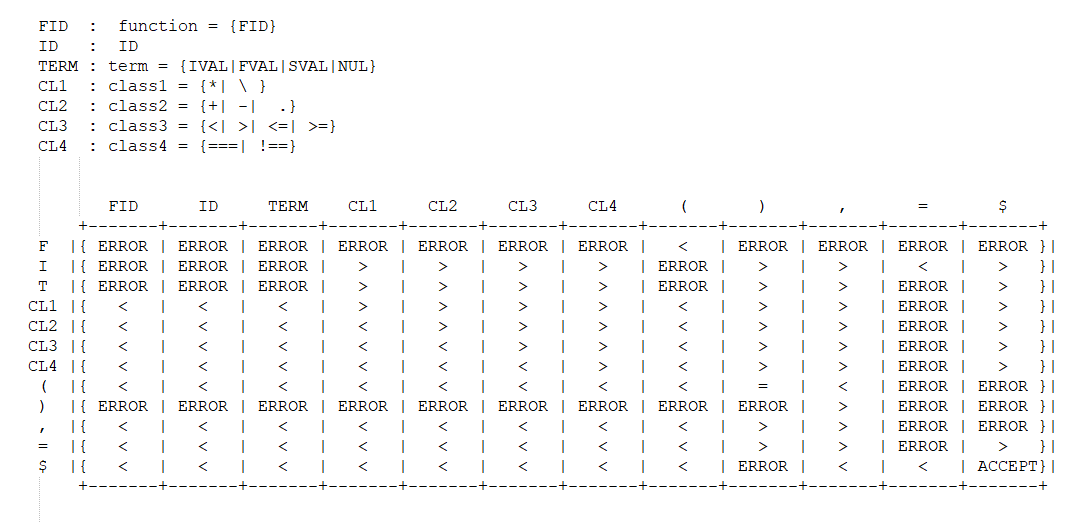
\includegraphics{diagrams/precedence_table.png}}
		\label{prec_table}
	\end{figure}
%%%
	\newpage
	
	\begingroup\centering
	\section*{Pravidla LL gramatiky}
	\label{gram}
	\endgroup
	\begin{lstlisting}[language=Python]
	prog -> PS_MARK PC_MARK prog_body

	prog_body -> body_part prog_body
	           | fun_def prog_body
	           | EPS
	
	prog_end -> PE_MARK EOS
	          | EOS
	
	body -> body_part body
	      | EPS
	
	body_part -> if_n
	           | while_n
	           | extended_expr
	           | ret
	
	extended_expr -> EXPR SEMIC 
	               | EXPR_FCALL SEMIC
	               | EXPR_PAR SEMIC
	               | EXPR_ASSIGN SEMIC
	
	ret -> RETURN ret_cont
	ret_cont -> EXPR SEMIC
	          | EXPR_PAR SEMIC
	          | EXPR_FCALL SEMIC
	          | SEMIC
	
	while_n -> WHILE EXPR_PAR LBRC body RBRC
	
	if_n -> IF EXPR_PAR LBRC body RBRC else_n
	else_n -> ELSE LBRC body RBRC
	        | EPS
		  
	fun_def -> FUNC F_ID LPAR par_list RPAR TYPE ret_type LBRC fun_body RBRC
	
	par_list -> type_n ID par_list_cont
	          | EPS
	
	par_list_cont -> COMMA par_list
	               | EPS
				
	ret_type -> type_n
	          | VTYPE
	
	type_n -> STYPE
	        | ITYPE
		| FTYPE
		| NSTYPE
		| NITYPE
		| NFTYPE

	\end{lstlisting}

%%%

\end{document}
